\documentclass[12pt, a4paper]{article}

% ===== 中文支持 =====
\usepackage[UTF8, zihao=-4]{ctex}

% ===== 页边距 =====
\usepackage[top=2.5cm, bottom=2.5cm, left=2.8cm, right=2.8cm]{geometry}

% ===== 字体 =====
\usepackage{fontspec}
\setmainfont{Times New Roman}

% ===== 行距 =====
\usepackage{setspace}
\setstretch{1.5}
\setlength{\parskip}{0pt}

% ===== 插图 =====
\usepackage{graphicx}
\usepackage{float}
\graphicspath{{./}}

% ===== 表格 =====
\usepackage{booktabs}
\usepackage{array}
\usepackage{multirow}

% ===== 数学公式 =====
\usepackage{amsmath, amssymb}

% ===== 图表编号（分章） =====
\usepackage{chngcntr}
\counterwithin{figure}{section}
\counterwithin{table}{section}
\renewcommand{\thefigure}{\arabic{section}-\arabic{figure}}
\renewcommand{\thetable}{\arabic{section}-\arabic{table}}

% ===== 图表标题格式 =====
\usepackage{caption}
\captionsetup{
  font=small,
  labelsep=space,
  justification=centering,
  aboveskip=6pt,
  belowskip=12pt
}
\captionsetup[table]{
  aboveskip=12pt,
  belowskip=6pt,
  position=above
}

% ===== 页眉页脚 =====
\usepackage{fancyhdr}
\setlength{\headheight}{15pt}
\pagestyle{fancy}
\fancyhf{}
\fancyhead[C]{\small 光栅参数测量实验报告}
\fancyfoot[C]{\small\thepage}

% ===== 超链接 =====
\usepackage[colorlinks=true, linkcolor=black, citecolor=black, urlcolor=blue,
            bookmarks=true, bookmarksnumbered=true]{hyperref}

% ===== 章节标题格式 =====
\usepackage{titlesec}
\titleformat{\section}[block]
  {\centering\heiti\zihao{4}}{\thesection}{1em}{}
\titlespacing*{\section}{0pt}{24pt}{18pt}
\titleformat{\subsection}[hang]
  {\heiti\zihao{-4}}{\thesubsection}{1em}{}
\titlespacing*{\subsection}{0pt}{18pt}{6pt}
\titleformat{\subsubsection}[hang]
  {\heiti\zihao{-4}}{\thesubsubsection}{1em}{}
\titlespacing*{\subsubsection}{0pt}{12pt}{6pt}

\begin{document}

% ===== 封面 =====
\begin{titlepage}
  \centering
  \vspace*{3cm}
  {\heiti\zihao{2} 实验报告} \\[1cm]
  {\heiti\zihao{3} 光栅参数测量实验} \\[2cm]
  \begin{tabular}{ll}
    姓\quad 名： & 叶哲昊 \\[0.5cm]
    学\quad 号： & 24012561 \\[0.5cm]
    实验桌号：   & B3 \\[0.5cm]
    合作者：     & 邓宇明（24012586）\\[0.5cm]
    实验日期：   & 2026年4月17日 \\
  \end{tabular}
  \vfill
\end{titlepage}

\tableofcontents
\newpage

\setcounter{page}{1}

% ==============================
\section{实验目的}
% ==============================

\begin{enumerate}
  \item 了解衍射光栅（diffraction grating）的基本结构及工作原理，掌握光栅方程的推导与应用。
  \item 搭建光路，利用透射光栅的夫朗和费（Fraunhofer）衍射，通过测量各级衍射亮斑位置计算光栅常数~$d$。
  \item 比较不同衍射级次对测量精度的影响，分析误差来源。
  \item 利用标准光栅（100~L/mm）对激光波长进行反算，并计算各级次相对误差，加深对光栅方程的理解。
  \item 观察改变聚焦透镜与白屏距离、改变通光孔大小对衍射图案的影响。
\end{enumerate}


% ==============================
\section{实验原理}
% ==============================

\subsection{衍射光栅}

衍射光栅是由大量等宽、等间距、平行排列的狭缝构成的光学元件。设透光部分宽度为~$a$，不透光部分宽度为~$b$，则光栅常数定义为：

\begin{equation}
  d = a + b
\end{equation}

光栅可按调制方式（振幅型与相位型）、工作方式（透射型与反射型）、表面形状（平面光栅与凹面光栅）等进行分类。本实验使用的是透射型全息光栅。

\subsection{光栅方程}

当单色平行光垂直入射到光栅平面时，各缝衍射光在衍射角~$\theta$~方向发生多光束干涉，主极大出现的条件（光栅方程）为：

\begin{equation}
  d \sin\theta = m\lambda \qquad m = 0, \pm1, \pm2, \cdots
\end{equation}

其中 $d$ 为光栅常数，$\theta$ 为衍射角，$m$ 为衍射级次，$\lambda$ 为入射光波长。

当入射光以倾斜角~$i$~入射时，一般光栅方程修正为：

\begin{equation}
  d(\sin\theta \pm \sin i) = m\lambda
\end{equation}

\subsection{多缝衍射强度分布}

$N$~缝衍射的合成光强为单缝衍射因子与多光束干涉因子之积：

\begin{equation}
  I = I_0 \left(\frac{\sin\alpha}{\alpha}\right)^2 \cdot
      \left[\frac{\sin(N\delta/2)}{\sin(\delta/2)}\right]^2
\end{equation}

其中

\[
  \alpha = \frac{\pi a \sin\theta}{\lambda}, \qquad
  \delta = \frac{2\pi d \sin\theta}{\lambda}
\]

主极大出现于 $d\sin\theta = m\lambda$，其强度为 $N^2 I_0\bigl(\tfrac{\sin\alpha}{\alpha}\bigr)^2$，较单缝提高 $N^2$ 倍。相邻主极大之间有 $N-1$ 个零值，主极大半角宽度为：

\begin{equation}
  \Delta\theta = \frac{\lambda}{Nd\cos\theta}
\end{equation}

缝数 $N$ 越大，衍射条纹越细锐。

\subsection{实验一测量原理}

\begin{figure}[H]
  \centering
  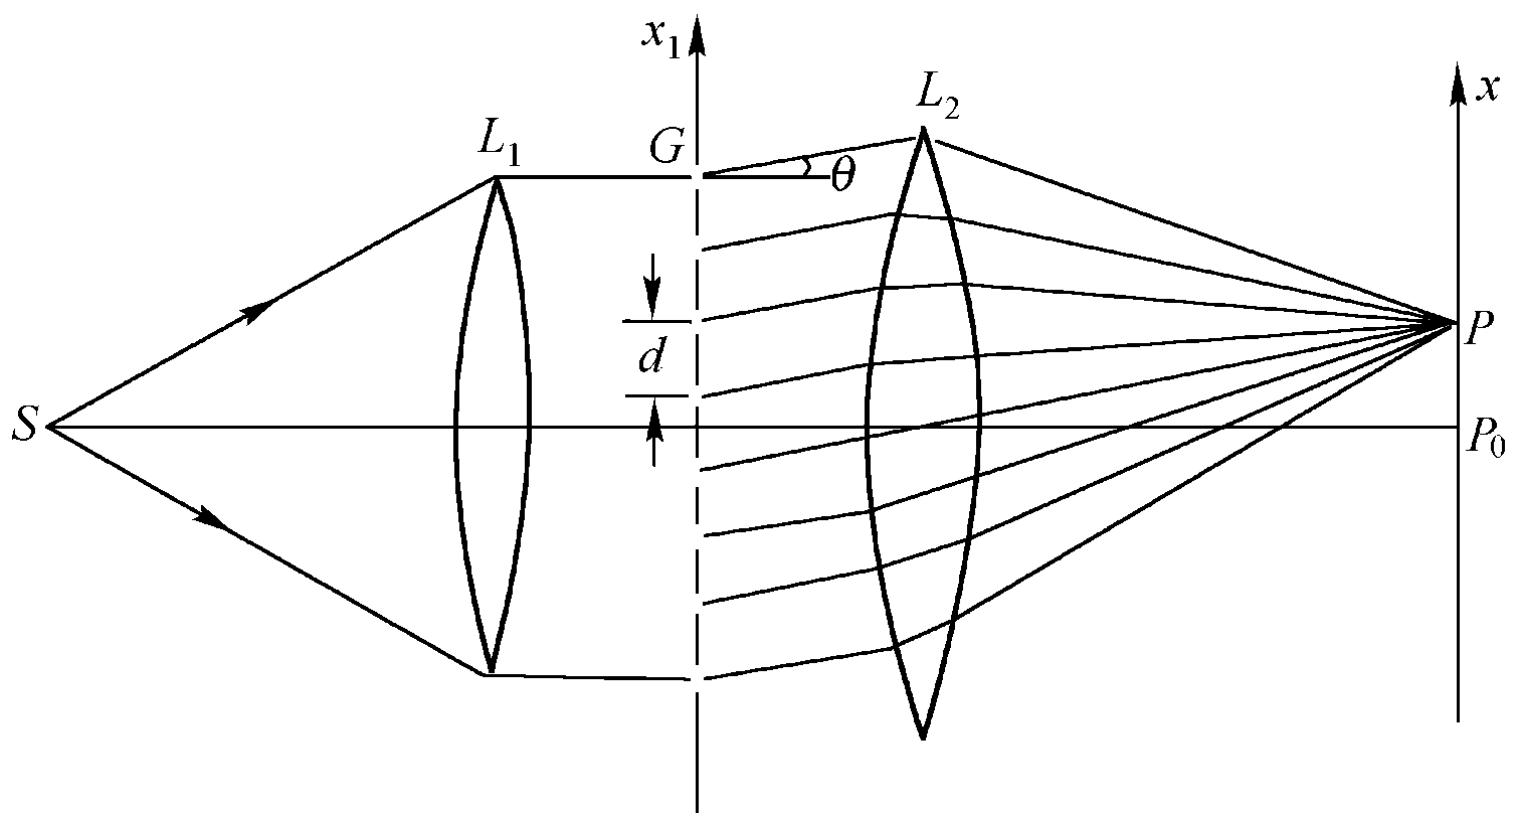
\includegraphics[width=0.75\textwidth]{images/856003ec387dfc0c3b1111df9a6ed0394fea84be949b88c8371d36cb6a65a37e.jpg}
  \caption{实验一光路原理图（$S$：点光源，$L_1$：准直透镜，$G$：光栅，$L_2$：聚焦透镜，$P_0/P$：观察屏）}
  \label{fig:optical-path-1}
\end{figure}

如图~\ref{fig:optical-path-1}~所示，激光经空间滤波器与准直透镜~$L_1$~展开为均匀平行光后，垂直照射透射光栅~$G$，衍射光经聚焦透镜~$L_2$~汇聚于焦平面白屏上，形成一系列分立亮斑。

设聚焦透镜焦距为~$f$（即光栅至白屏距离~$L$），第~$m$~级衍射斑到零级斑的距离为~$x_m$，则：

\begin{equation}
  \tan\theta_m = \frac{x_m}{L}
\end{equation}

由此得衍射角~$\theta_m = \arctan(x_m/L)$，代入光栅方程即可求得光栅常数：

\begin{equation}
  d = \frac{m\lambda}{\sin\theta_m}
  \label{eq:grating-constant}
\end{equation}

\subsection{实验二测量原理}

\begin{figure}[H]
  \centering
  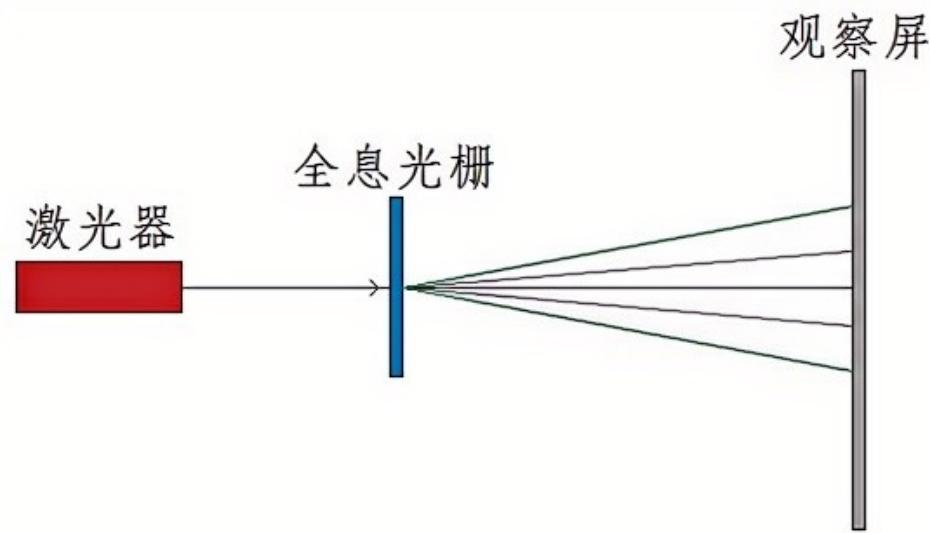
\includegraphics[width=0.65\textwidth]{images/0e3728f23ed6006c4d049f8d8a6929e56a3ebf5ba3ccdd0d81259216abfe1353.jpg}
  \caption{实验二光路原理图（激光器直接照射全息光栅，用卷尺量取光栅到观察屏距离）}
  \label{fig:optical-path-2}
\end{figure}

如图~\ref{fig:optical-path-2}~所示，激光束经衰减片后直接照射光栅，用卷尺量取光栅到白屏的距离~$L$，在白屏刻度尺上读取~$\pm1$~级衍射光斑到零级光斑的距离~$x$，计算衍射角后代入式~(\ref{eq:grating-constant})~求得光栅常数。


% ==============================
\section{实验仪器}
% ==============================

\begin{enumerate}
  \item 绿色半导体激光器（$\lambda = 532~\text{nm}$）
  \item 光学衰减片
  \item 空间滤波器（小孔光阑 + 显微物镜组合）
  \item 准直透镜~$L_1$
  \item 可调光阑（通光孔可调节）
  \item 透射全息光栅（标称光栅线数~$100~\text{L/mm}$，$d = 10~\mu\text{m}$）
  \item 聚焦透镜~$L_2$
  \item 带刻度白屏（量程~0\textasciitilde9~cm，分度值~0.5~mm）
  \item 光学导轨与支架
  \item 卷尺
\end{enumerate}

% ==============================
\section{实验步骤}
% ==============================

\subsection{实验一：多级衍射法测光栅常数}

\begin{enumerate}
  \item 在光学导轨上依次安装激光器、衰减片、空间滤波器、准直透镜~$L_1$、可调光阑、透射光栅、聚焦透镜~$L_2$~和白屏，调节各元件共轴等高。
  \item 开启激光器，调节空间滤波器至激光束被均匀扩束，再经准直透镜变为平行光束，使其垂直正入射到光栅平面。
  \item 调节白屏与~$L_2$~之间的距离至合适位置，使~$\pm1$\textasciitilde$\pm5$~级共11个衍射亮斑清晰成像于白屏刻度尺范围内。
  \item 读取各级衍射亮斑（$k = -5, -4, \cdots, 0, \cdots, +4, +5$）的位置坐标~$x_k$（cm）及光栅到白屏距离~$L$（cm），记录零级位置~$x_0$。
  \item 拍摄光路实物图及衍射图案照片留存。
  \item 改变白屏与~$L_2$~之间的距离，观察并记录衍射图案变化特点。
  \item 调节可调光阑改变照射光栅的通光孔大小，观察并记录衍射图案变化特点。
\end{enumerate}

\subsection{实验二：直接法测光栅常数}

\begin{enumerate}
  \item 拆去准直透镜和聚焦透镜，仅保留激光器、衰减片和光栅，使激光束直接照射光栅。
  \item 用卷尺量取光栅到白屏的距离~$L$（cm）。
  \item 在白屏刻度上读取~$+1$~级和~$-1$~级衍射光斑到零级光斑的距离，计算平均值~$\bar{x}$（cm）。
  \item 改变光栅到白屏的距离，重复测量，共取两组数据。
  \item 拍摄光路实物图。
\end{enumerate}

\subsection{实验三：利用标准光栅测量激光波长}

\begin{enumerate}
  \item 使用实验一的光路与数据（光栅线数~100~L/mm，$d = 10000~\text{nm}$）。
  \item 利用各级衍射角代入~$\lambda = d\sin\theta_k / k$~计算各级次对应的激光波长。
  \item 计算各级次测量波长的绝对误差~$\Delta\lambda = |\lambda - \lambda_0|$ 和相对误差~$E = \Delta\lambda/\lambda_0 \times 100\%$（取~$\lambda_0 = 532~\text{nm}$）。
  \item 对比分析各衍射级次的测量精度。
\end{enumerate}


% ==============================
\section{实验数据与处理}
% ==============================

\subsection{实验一：多级衍射法}

实验参数：激光波长~$\lambda = 532~\text{nm}$，光栅到白屏距离~$L = 15.10~\text{cm}$，零级光斑位置~$x_0 = 4.52~\text{cm}$。

各级衍射亮斑的位置读数及光栅常数计算结果见表~\ref{tab:exp1}。

\begin{table}[H]
  \centering
  \caption{实验一各级衍射亮斑测量数据及光栅常数计算结果}
  \label{tab:exp1}
  \resizebox{\linewidth}{!}{%
  \begin{tabular}{ccccccc}
    \toprule
    级次~$k$ & 位置读数~$x$~(cm) & 到中心距~$|x-x_0|$~(cm) &
    $\tan\theta = |x-x_0|/L$ & 衍射角~$\theta$~($^\circ$) &
    $\sin\theta$ & 光栅常数~$d$~(nm) \\
    \midrule
    $-5$ & 0.69 & 3.83 & 0.2536 & 14.23 & 0.2457 & 10819 \\
    $-4$ & 1.41 & 3.11 & 0.2060 & 11.64 & 0.2016 & 10548 \\
    $-3$ & 2.15 & 2.37 & 0.1570 &  8.92 & 0.1550 & 10293 \\
    $-2$ & 2.94 & 1.58 & 0.1046 &  5.97 & 0.1041 & 10224 \\
    $-1$ & 3.71 & 0.81 & 0.0536 &  3.07 & 0.0536 &  9932 \\
     $0$ & 4.52 & 0    & 0      &  0    & 0      & ---   \\
    $+1$ & 5.31 & 0.79 & 0.0523 &  3.00 & 0.0523 & 10182 \\
    $+2$ & 6.10 & 1.58 & 0.1046 &  5.97 & 0.1041 & 10224 \\
    $+3$ & 6.88 & 2.36 & 0.1563 &  8.90 & 0.1547 & 10316 \\
    $+4$ & 7.64 & 3.12 & 0.2066 & 11.67 & 0.2022 & 10517 \\
    $+5$ & 8.38 & 3.86 & 0.2556 & 14.34 & 0.2476 & 10740 \\
    \bottomrule
  \end{tabular}}
\end{table}

对10组（除零级外）光栅常数取平均：

\begin{multline}
  \bar{d}_1 = \frac{1}{10}\sum_{k} d_k \\
  = \frac{10819 + 10548 + 10293 + 10224 + 9932 + 10182 + 10224 + 10316 + 10517 + 10740}{10} \\
  = 10379.5~\text{nm}
\end{multline}

\textbf{实验一结果：}$\bar{d}_1 = 10379.5~\text{nm} \approx 10.38~\mu\text{m}$，对应光栅线数~$N_1 = 1/\bar{d}_1 = 96.3~\text{线/mm}$。

\subsection{实验二：直接法}

实验参数：激光波长~$\lambda = 532~\text{nm}$，测量级次~$k = \pm1$。两次测量数据见表~\ref{tab:exp2}。

\begin{table}[H]
  \centering
  \caption{实验二测量数据及光栅常数计算结果}
  \label{tab:exp2}
  \resizebox{\linewidth}{!}{%
  \begin{tabular}{ccccccccccc}
    \toprule
    次数 & $L$~(cm) & $x_{+1}$~(cm) & $x_{-1}$~(cm) & $x_0$~(cm) &
    $|x_{+1}-x_0|$ & $|x_{-1}-x_0|$ & $\bar{x}$~(cm) &
    $\tan\theta$ & $\theta$~($^\circ$) & $d$~(nm) \\
    \midrule
    1 & 10.93 & 5.13 & 3.98 & 4.55 & 0.58 & 0.57 & 0.575 & 0.0526 & 3.01 & 10126 \\
    2 & 16.54 & 5.24 & 3.50 & 4.48 & 0.76 & 0.98 & 0.870 & 0.0526 & 3.01 & 10128 \\
    \midrule
    均值 & --- & --- & --- & --- & --- & --- & 0.723 & 0.0526 & 3.01 & 10127 \\
    \bottomrule
  \end{tabular}}
\end{table}

\textbf{实验二结果：}$\bar{d}_2 = 10127~\text{nm} \approx 10.13~\mu\text{m}$，对应光栅线数~$N_2 = 98.7~\text{线/mm}$。

\subsection{实验三：利用标准光栅反算激光波长}

标准光栅参数：$d = 10000~\text{nm}$（100~L/mm）。使用实验一数据（$L = 15.10~\text{cm}$），各级次波长计算结果见表~\ref{tab:exp3}。

\begin{table}[H]
  \centering
  \caption{实验三各级次波长测量及误差分析（$\lambda_0 = 532~\text{nm}$，$d = 10000~\text{nm}$）}
  \label{tab:exp3}
  \small
  \begin{tabular}{ccccccc}
    \toprule
    级次~$k$ & $|x-x_0|$~(cm) & $\tan\theta$ & $\theta$~($^\circ$) & $\sin\theta$ &
    $\lambda = d\sin\theta/|k|$~(nm) & 相对误差~$E$~(\%) \\
    \midrule
    $-5$ & 3.83 & 0.2536 & 14.23 & 0.2457 & 491.4 & 7.63 \\
    $-4$ & 3.11 & 0.2060 & 11.64 & 0.2016 & 504.0 & 5.26 \\
    $-3$ & 2.37 & 0.1570 &  8.92 & 0.1550 & 516.7 & 2.88 \\
    $-2$ & 1.58 & 0.1046 &  5.97 & 0.1041 & 520.5 & 2.16 \\
    $-1$ & 0.81 & 0.0536 &  3.07 & 0.0536 & 536.0 & 0.75 \\
    $+1$ & 0.79 & 0.0523 &  3.00 & 0.0523 & 523.0 & 1.69 \\
    $+2$ & 1.58 & 0.1046 &  5.97 & 0.1041 & 520.5 & 2.16 \\
    $+3$ & 2.36 & 0.1563 &  8.90 & 0.1547 & 515.7 & 3.06 \\
    $+4$ & 3.12 & 0.2066 & 11.67 & 0.2022 & 505.5 & 4.98 \\
    $+5$ & 3.86 & 0.2556 & 14.34 & 0.2476 & 495.2 & 6.92 \\
    \bottomrule
  \end{tabular}
\end{table}

计算公式：$\lambda = d\sin\theta / |k|$，$E = |\lambda - 532|/532 \times 100\%$。

\textbf{实验三结果：}平均测量波长~$\bar{\lambda} = 513.8~\text{nm}$；最小相对误差出现在~$k = -1$~级，$E = 0.75\%$；最大相对误差出现在~$k = -5$~级，$E = 7.63\%$。


% ==============================
\section{实验结果与分析}
% ==============================

\subsection{实验光路照片}

\begin{figure}[H]
  \centering
  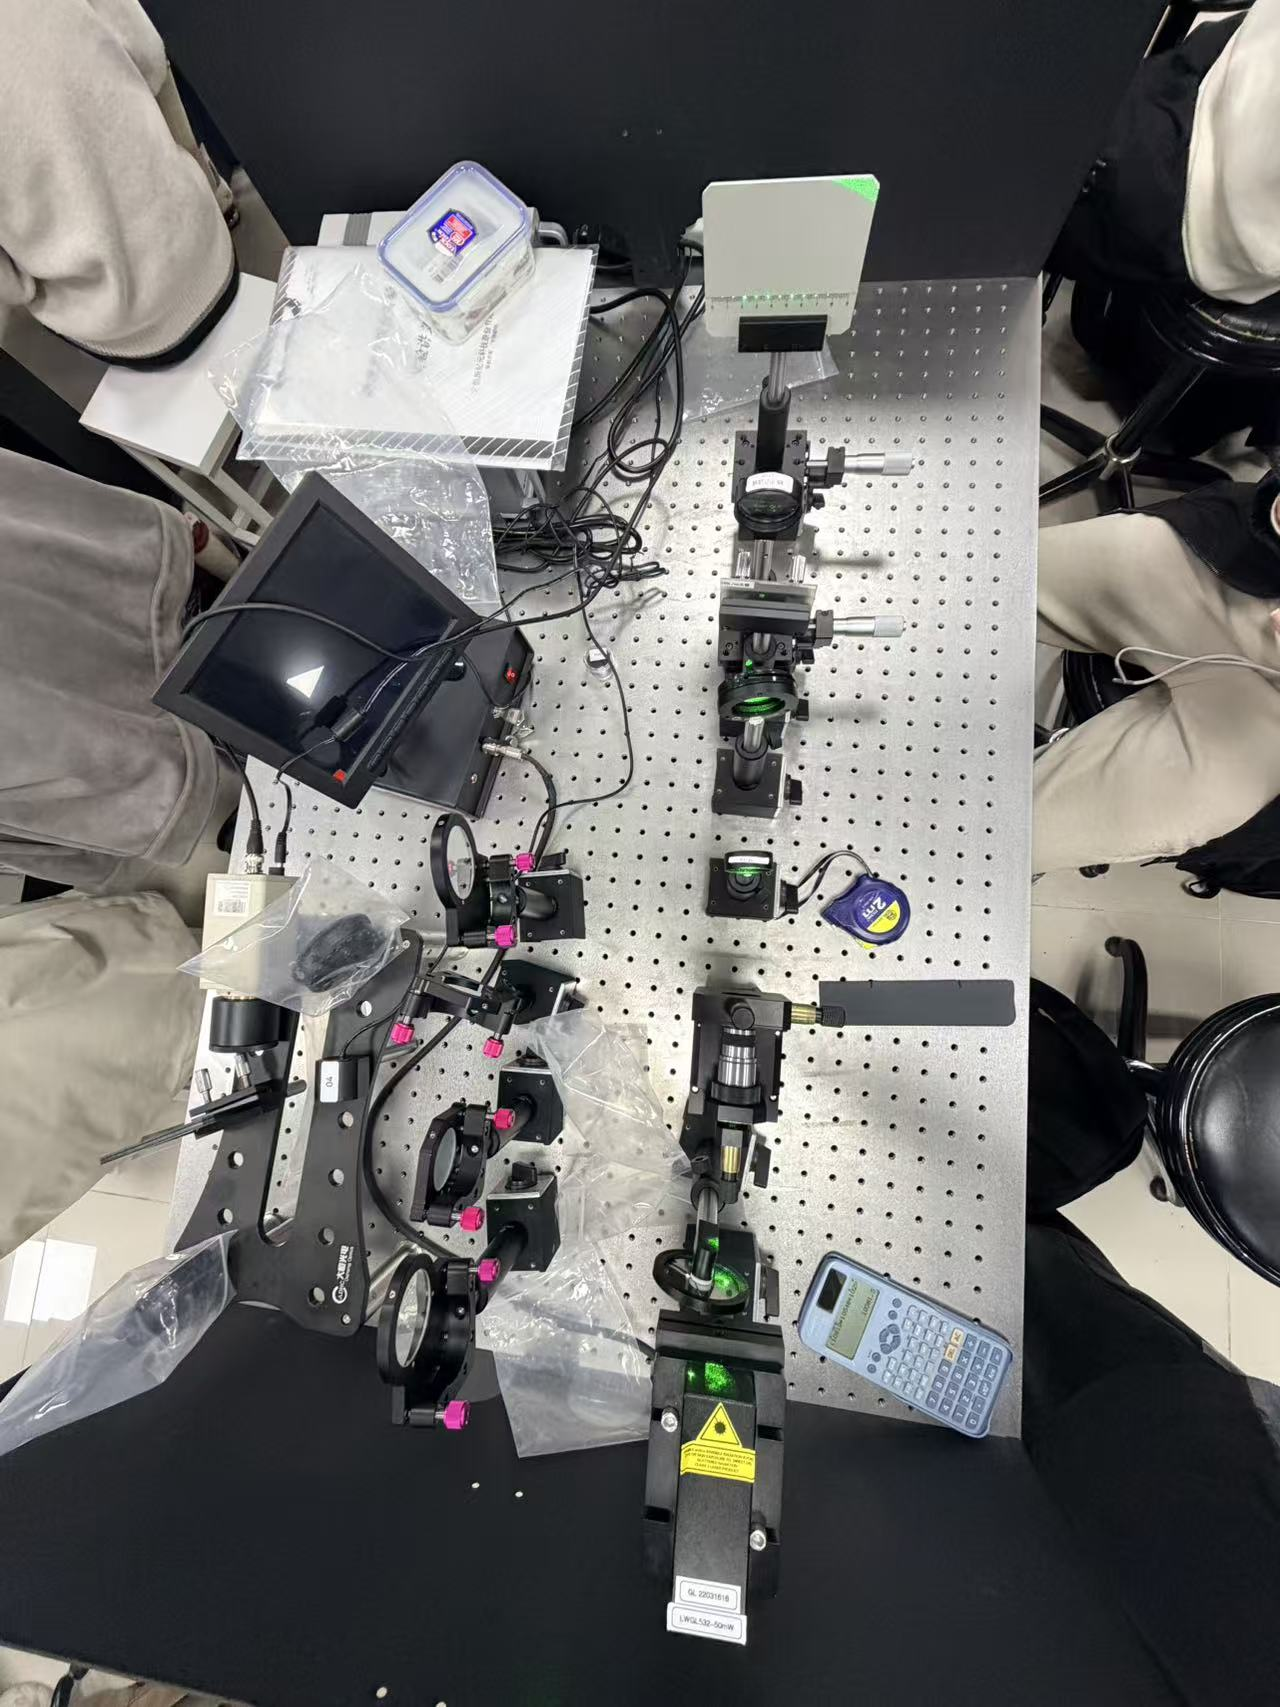
\includegraphics[width=0.72\textwidth]{实验图片/实验一装置完整实物光路搭建.jpg}
  \caption{实验一完整实物光路搭建（激光器—衰减片—空间滤波器—准直镜—光阑—光栅—聚焦透镜—白屏）}
  \label{fig:setup1}
\end{figure}

\begin{figure}[H]
  \centering
  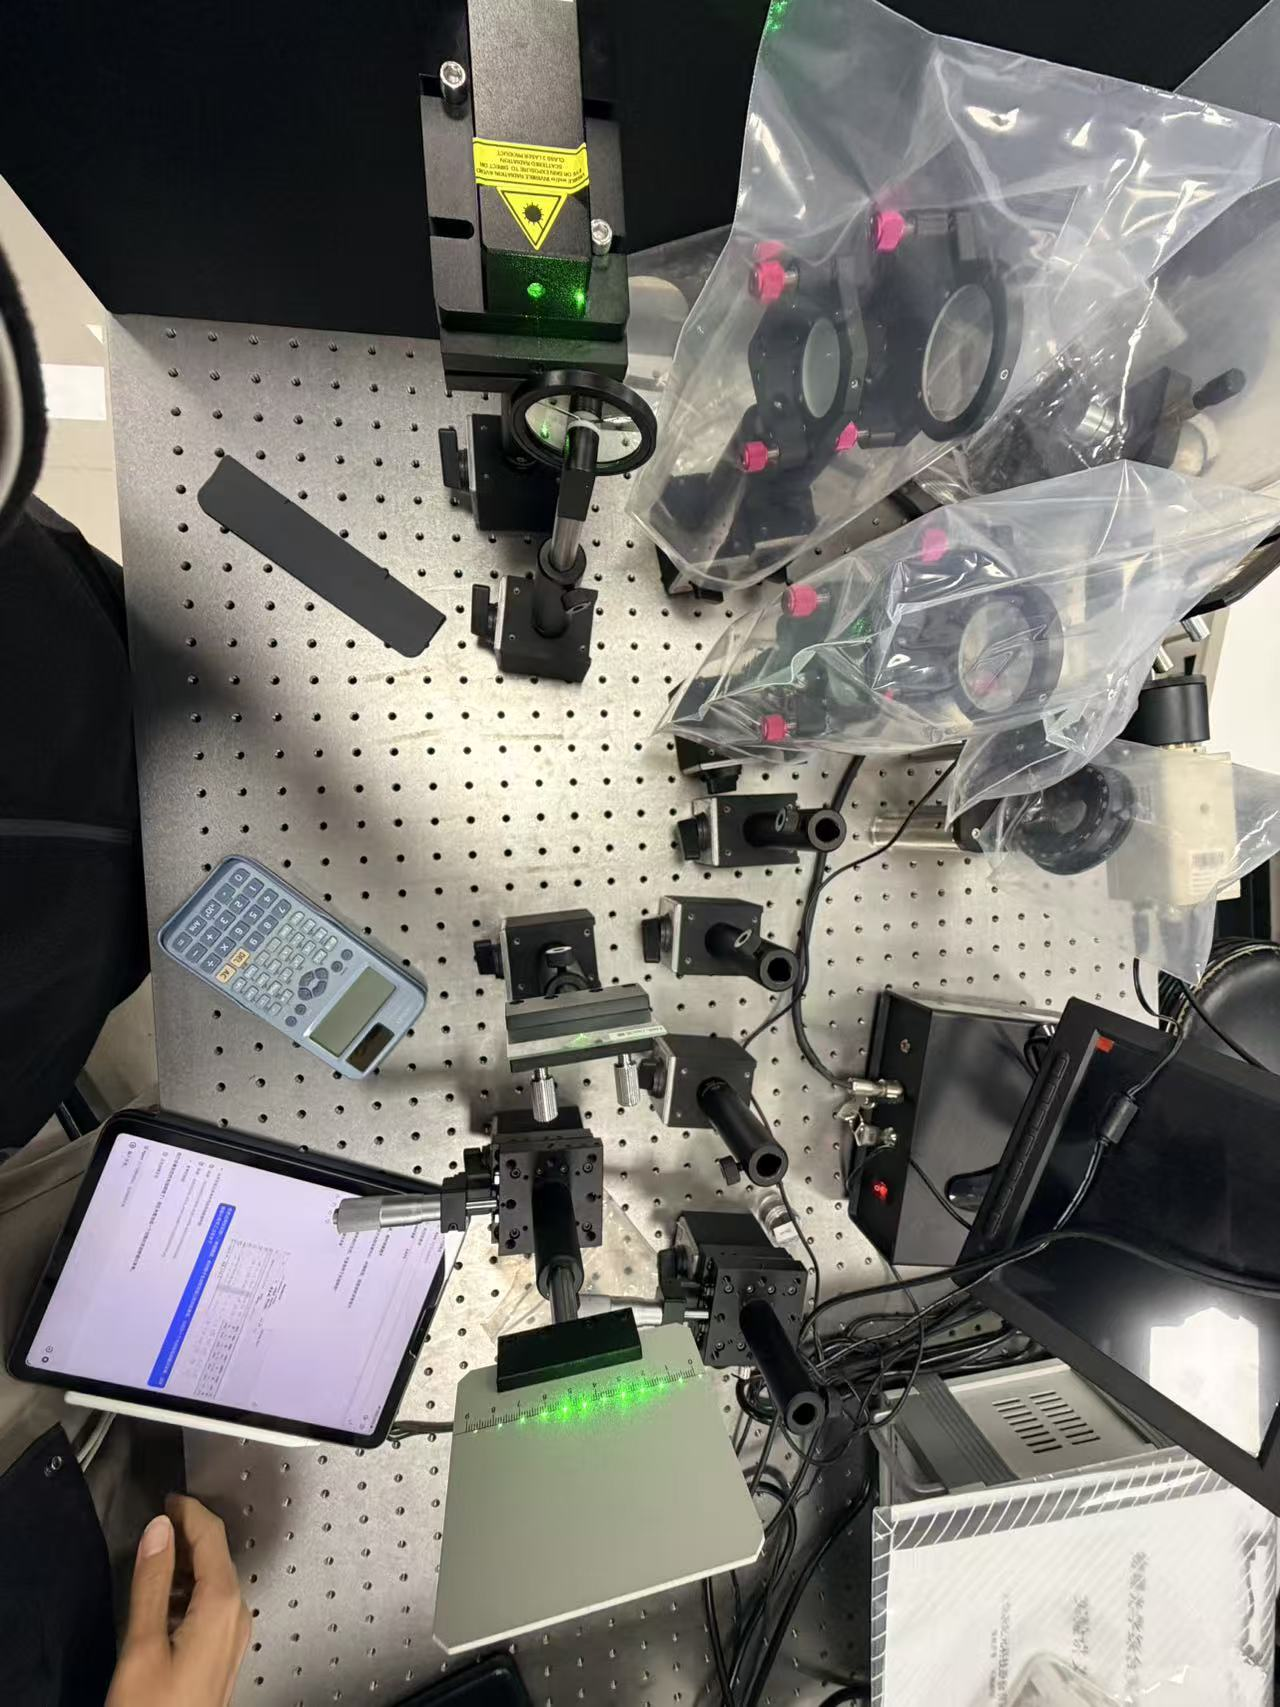
\includegraphics[width=0.72\textwidth]{实验图片/实验二光路搭建.jpg}
  \caption{实验二光路搭建（激光器—衰减片—光栅—白屏，不含透镜）}
  \label{fig:setup2}
\end{figure}

\subsection{衍射图案观察}

图~\ref{fig:big-aperture} 与图~\ref{fig:small-aperture}~分别展示了在白屏置于聚焦透镜焦平面时，可调光阑通光孔较大和较小时的衍射图案。

\begin{figure}[H]
  \centering
  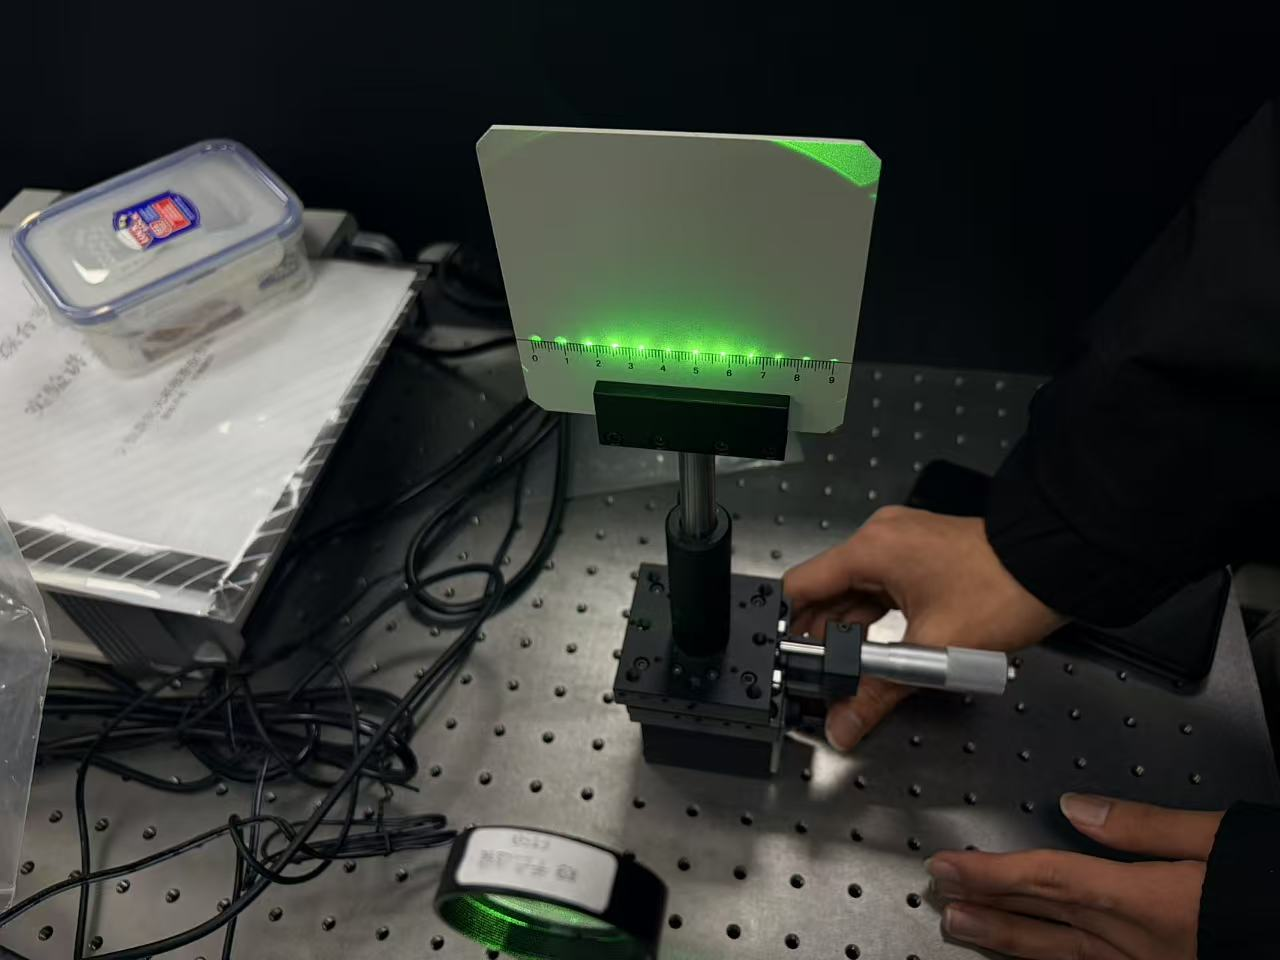
\includegraphics[width=0.70\textwidth]{实验图片/在白屏放在焦平面上时，调节通光孔几乎不会改变衍射图案（略微变大），这是大的场景.jpg}
  \caption{焦平面处通光孔较大时的衍射图案（亮斑排列清晰，11个亮斑可见）}
  \label{fig:big-aperture}
\end{figure}

\begin{figure}[H]
  \centering
  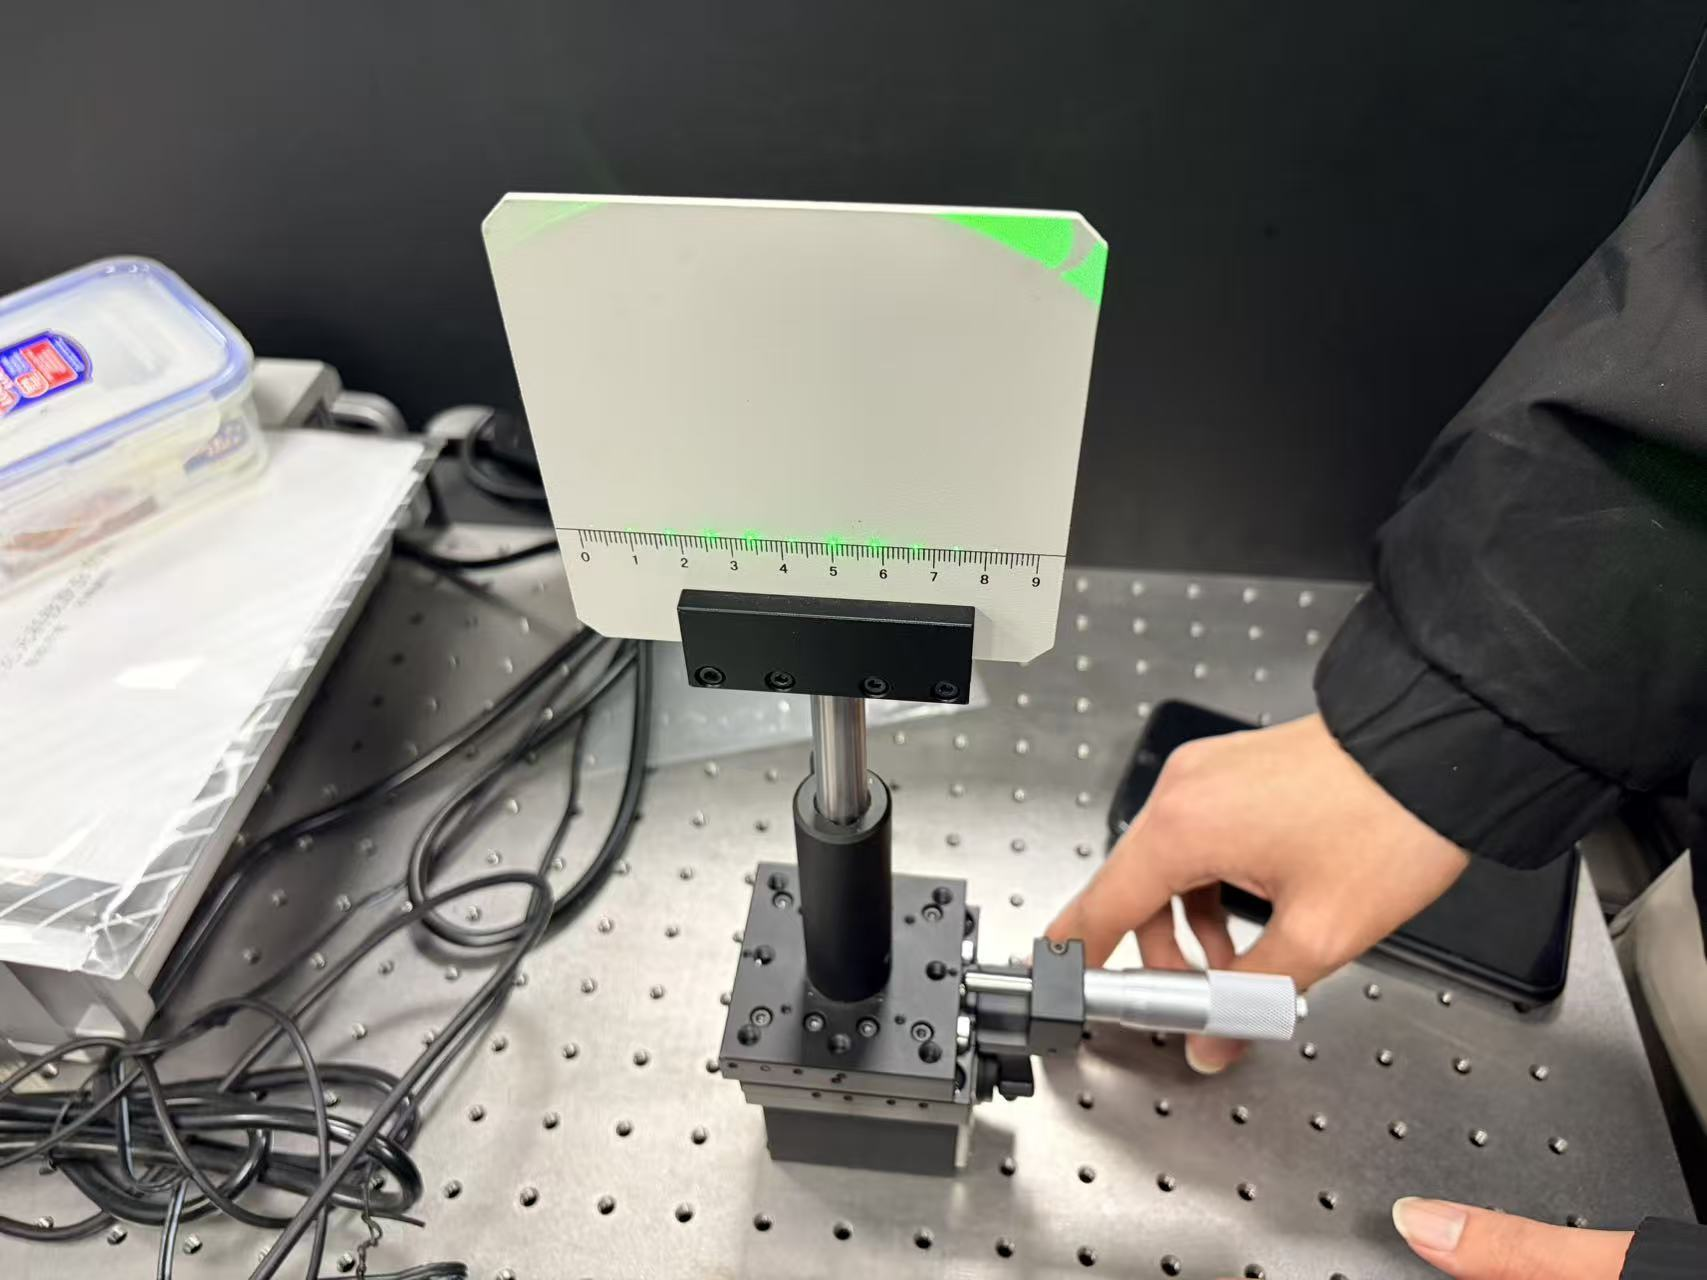
\includegraphics[width=0.70\textwidth]{实验图片/在白屏放在焦平面上时，调节通光孔几乎不会改变衍射图案（略微变大），这是小的场景.jpg}
  \caption{焦平面处通光孔较小时的衍射图案（亮斑略微收窄，相对误差变化不明显）}
  \label{fig:small-aperture}
\end{figure}

\begin{figure}[H]
  \centering
  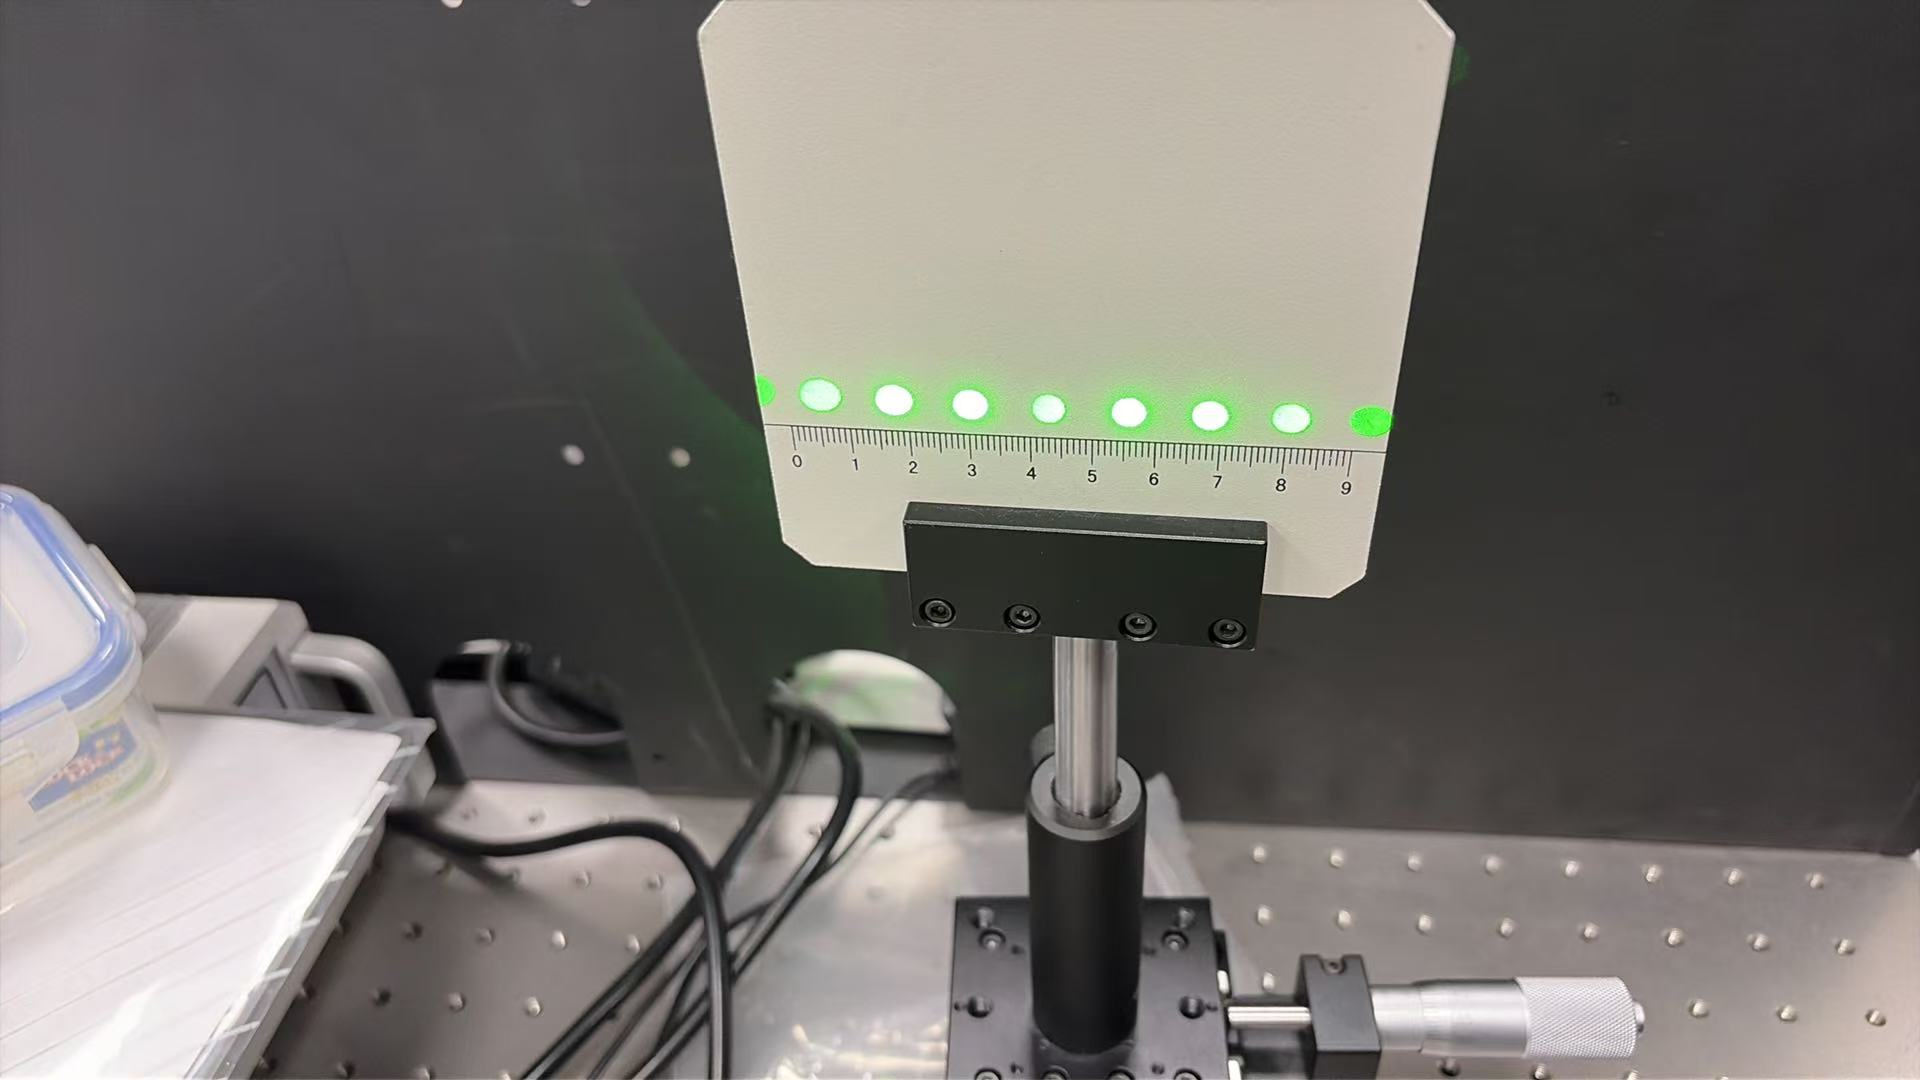
\includegraphics[width=0.70\textwidth]{实验图片/改变白屏与聚焦透镜的距离记录并对比光栅衍射图案的特点，距离拉长之后出现的效果：不再聚焦，变为光斑.jpg}
  \caption{白屏偏离焦平面后衍射图案变化：亮斑不再聚焦，扩散为弥散光斑}
  \label{fig:defocused}
\end{figure}

\subsection{现象分析}

\textbf{改变屏与透镜距离的影响：}当白屏恰好位于聚焦透镜~$L_2$~的焦平面上时，各级平行衍射光汇聚为最小、最亮的衍射亮斑，如图~\ref{fig:big-aperture}~所示，共可见~$0, \pm1, \pm2, \pm3, \pm4, \pm5$~共11个亮斑。当白屏位置偏离焦平面（如图~\ref{fig:defocused}），各级光束未充分会聚，亮斑弥散为大光斑，不利于读数。

\textbf{改变通光孔大小的影响：}在白屏置于焦平面的条件下，调节可调光阑改变照射到光栅上的光束截面积，对焦平面处衍射亮斑的角位置几乎无影响（衍射角由光栅常数和波长决定），但亮斑亮度随光束截面积增大而增强，如图~\ref{fig:big-aperture}~与图~\ref{fig:small-aperture}~对比所示。

\textbf{各实验方案比较：}实验一利用多个级次（$k = \pm1$\textasciitilde$\pm5$）的衍射亮斑位置计算光栅常数，结果平均值为~$\bar{d}_1 = 10379.5~\text{nm}$，与标称值~$10000~\text{nm}$~相对偏差约~3.8\%，测量较为准确。实验二仅利用~$\pm1$~级，两次测量结果分别为~$d_1 = 10126~\text{nm}$~和~$d_2 = 10128~\text{nm}$，两次结果高度一致，平均值~$\bar{d}_2 = 10127~\text{nm}$，与实验一结果及标称值吻合良好，验证了直接法的可靠性。

% ==============================
\section{误差分析}
% ==============================

\subsection{系统误差来源}

\begin{enumerate}
  \item \textbf{入射光非严格垂直于光栅平面：}若激光束与光栅法线存在夹角~$i$，则实际应使用斜入射光栅方程 $d(\sin\theta \pm \sin i) = m\lambda$，按正入射处理会引入系统误差；高级次（如~$\pm5$~级）的衍射角较大，该效应更显著。
  \item \textbf{聚焦透镜畸变与焦距不准：}$L_2$~的实际焦距与标称值存在偏差，导致~$L$~的确定存在系统误差；白屏未精确对准焦平面时亮斑弥散，读数引入误差。
  \item \textbf{光栅制造误差：}实际光栅常数与标称值（$10~\mu\text{m}$）之间存在制造偏差，导致实验三波长计算结果系统性偏低（平均~513.8~nm~而非~532~nm）。
\end{enumerate}

\subsection{随机误差来源}

\begin{enumerate}
  \item \textbf{白屏刻度读数误差：}刻度尺最小分度为~0.5~mm，读数不确定度约~$\pm0.25~\text{mm}$，对较低级次（$k = \pm1$）影响更显著，因~$x$~本身较小，相对误差大。
  \item \textbf{光斑中心判断不确定：}衍射亮斑有一定宽度，肉眼判断中心存在随机偏差。
  \item \textbf{光栅到白屏距离测量误差：}卷尺测量距离的读数偏差（约~$\pm1~\text{mm}$）对高级次影响较小，对低级次影响相对较大。
\end{enumerate}

\subsection{实验三误差规律分析}

由实验三数据（表~\ref{tab:exp3}）可知，低级次（$|k| = 1$）的衍射角~$\theta$~较小，$\sin\theta$~近似等于~$\tan\theta$，与实验一所用近似吻合，相对误差最小（约~0.75\%\textasciitilde1.69\%）；高级次（$|k| = 4, 5$）衍射角较大，$\sin\theta$~与~$\tan\theta$~偏差增大，且位置读数的绝对不确定度被放大，导致波长误差增大（达~5\%\textasciitilde7.63\%）。因此在利用单次测量求光栅常数时，中等级次（$|k| = 2, 3$）往往能在精度与灵敏度之间取得较好平衡。

% ==============================
\section{实验结论}
% ==============================

\begin{enumerate}
  \item 利用实验一（多级衍射法），成功测量了透射全息光栅的光栅常数：$\bar{d}_1 = 10379.5~\text{nm} \approx 10.38~\mu\text{m}$，对应光栅线数约~96.3~线/mm，与标称值~100~线/mm~相对偏差约~3.7\%，结果合理。
  \item 利用实验二（直接法，仅测~$\pm1$~级），两次测量结果均为~$\approx10127~\text{nm}$，与实验一结果（10379.5~nm）和标称值（10000~nm）相互印证，两种方法均证明该光栅常数约为~$10.1$	extasciitilde$10.4~\mu\text{m}$，对应线数~$97$	extasciitilde$99$~线/mm，与标称~100~线/mm~吻合。
  \item 实验三表明：利用标准光栅（$d = 10~\mu\text{m}$）对激光波长的反算精度随衍射级次升高而下降，低级次（$|k|=1$）误差最小（$\sim0.75\%$），高级次（$|k|=5$）误差最大（$\sim7.63\%$）。
  \item 观察实验现象得出：白屏须置于聚焦透镜焦平面方可使衍射亮斑最小最亮，便于精确读数；改变通光孔大小主要影响亮斑亮度，对衍射角位置影响极小，与理论预期一致。
  \item 光栅衍射实验中，提高测量精度的关键在于：保证激光垂直正入射、准确测定光栅到屏距离、以及合理选择测量级次。
\end{enumerate}

% ==============================
\section{思考题}
% ==============================

\subsection*{思考题1：光栅方程的前提条件及验证方法}

光栅方程 $d\sin\theta = k\lambda$ 成立的前提条件是：\textbf{单色平行光垂直入射到光栅平面}（即入射光方向与光栅平面的法线方向重合）。若入射光为非平行光或斜入射，则需改用斜入射光栅方程。

在本实验中，可通过以下方式检验该条件是否满足：

\begin{enumerate}
  \item \textbf{对称性检验：}观察白屏上各级衍射亮斑是否关于零级（$k=0$）中央亮斑左右严格对称，即 $+k$ 级与 $-k$ 级到零级的距离是否相等。若对称性良好，则说明入射光方向近似垂直于光栅面。
  \item \textbf{逐级计算一致性检验：}分别用 $+k$ 和 $-k$ 级数据各自代入 $d = k\lambda/\sin\theta$ 计算光栅常数，若两者结果接近，则满足垂直入射条件。
  \item \textbf{调节验证：}将光栅安装在转台上，微调光栅角度直至 $\pm1$ 级亮斑到零级的距离完全相等，此时即可认为满足垂直入射条件。
\end{enumerate}

\subsection*{思考题2：入射光不垂直于光栅平面对实验结果的影响}

若入射光以角度~$i$~斜入射，真实的光栅方程应为：

\begin{equation}
  d(\sin\theta - \sin i) = k\lambda
\end{equation}

若仍按正入射公式 $d\sin\theta = k\lambda$ 处理，将引入系统误差，具体表现为：

\begin{enumerate}
  \item \textbf{正负级次不再对称：}$+k$ 级与 $-k$ 级的衍射角大小不再相等，左侧和右侧测得的衍射角分别偏大和偏小（或反之），导致用 $+k$ 和 $-k$ 计算出的光栅常数出现系统偏差。
  \item \textbf{计算结果偏大或偏小：}以~$+k$~级为例，若斜入射使得 $\theta$ 偏大，则按正入射公式计算出的~$d$~将系统性偏大。
  \item \textbf{高级次误差更显著：}衍射角~$\theta$~越大，$\sin\theta$ 对角度的灵敏度越高，斜入射引起的 $\sin\theta$ 误差随级次升高而增大，因此高级次（$|k|=4,5$）的误差更为明显，与实验三中高级次相对误差较大的结果一致。
\end{enumerate}

实验中可通过取 $\pm k$ 级亮斑到零级距离的平均值来部分抵消斜入射引起的系统误差。

\subsection*{思考题3：两个透镜 $L_1$ 和 $L_2$ 的作用}

\begin{itemize}
  \item \textbf{$L_1$（准直透镜）的作用：}将激光器出射的发散光束（经空间滤波器小孔衍射后为球面波）变换为均匀的平行光束，保证照射到光栅上的光满足"平行光垂直入射"的前提条件，从而使光栅方程 $d\sin\theta = k\lambda$ 成立。若无 $L_1$，发散的球面波在光栅不同位置的入射角各不相同，衍射图案将严重弥散，无法精确测量各级衍射角。

  \item \textbf{$L_2$（聚焦透镜）的作用：}将沿同一衍射角~$\theta$~出射的平行衍射光汇聚到其焦平面上的一个点，形成清晰、细锐的衍射亮斑，便于在白屏上精确读取亮斑位置。与此同时，$L_2$~还起到"傅里叶变换"的光学作用——焦平面上各点的位置对应的正是不同衍射角~$\theta$，因此焦平面即为光栅的夫朗和费衍射场。若无~$L_2$，需将白屏放置在极远处（趋于无穷）才能观察到夫朗和费衍射图样，实验操作极为不便。
\end{itemize}

\appendix
\renewcommand{\thefigure}{\Alph{section}-\arabic{figure}}
\renewcommand{\thetable}{\Alph{section}-\arabic{table}}
\setcounter{figure}{0}
\setcounter{table}{0}

\section{原始数据记录}

下图为本实验现场记录的完整数据记录单原件，含指导教师签字确认，作为实验数据真实性的原始凭证。报告正文"实验数据与处理"章节中的所有测量数据均忠实誊录自该记录单。

\begin{figure}[H]
  \centering
  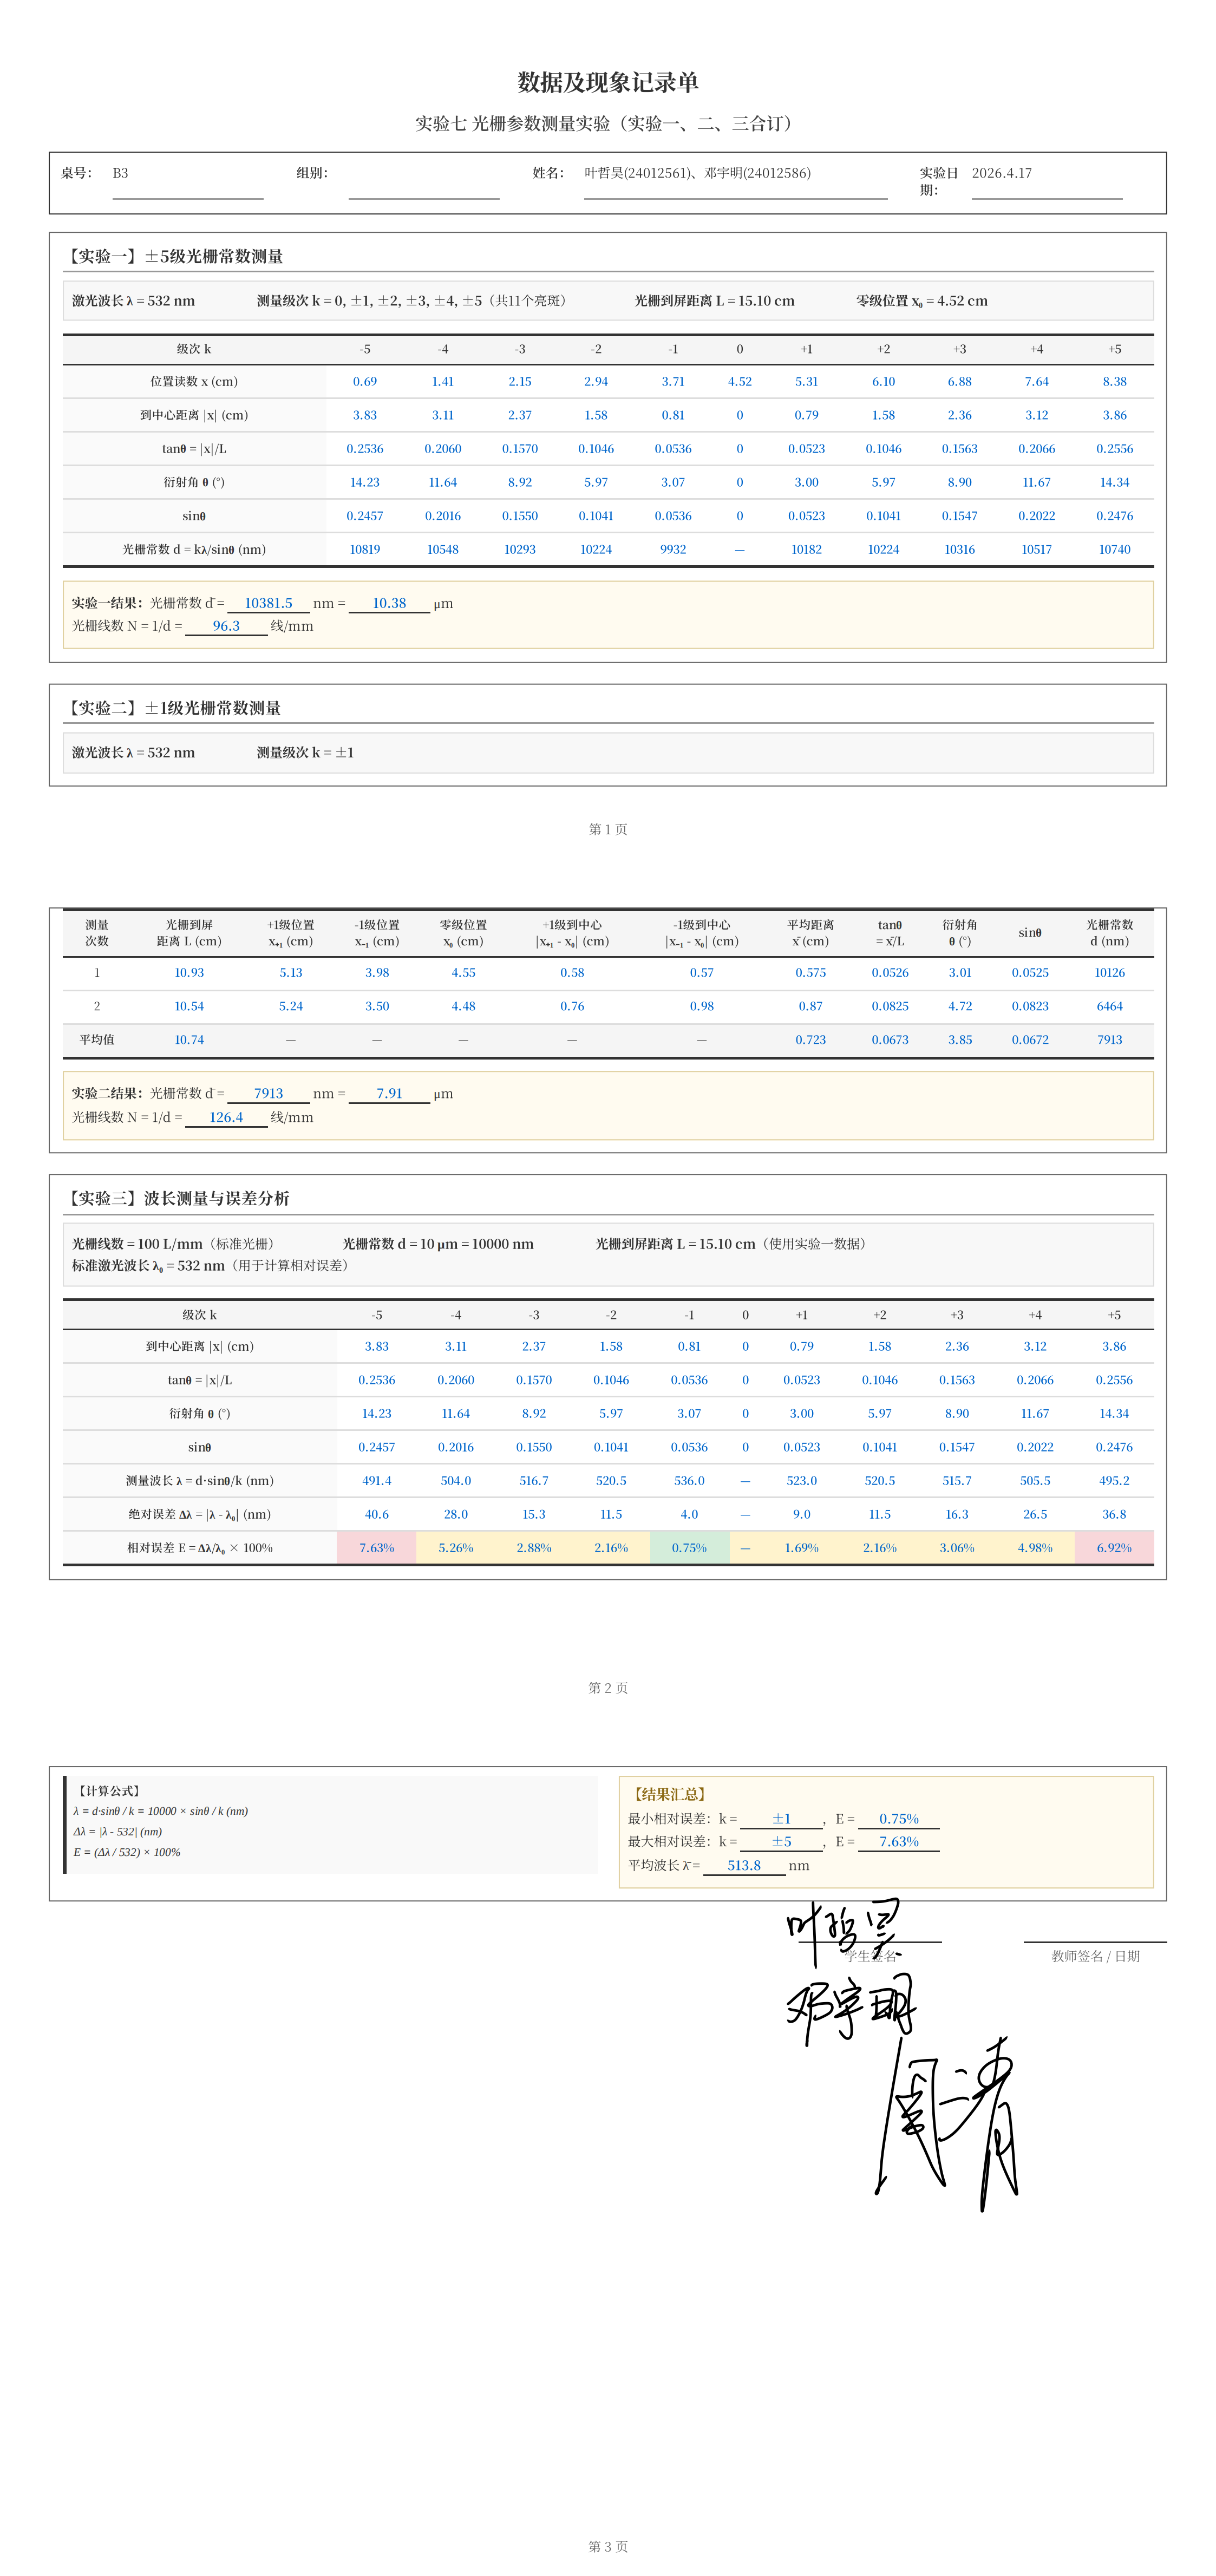
\includegraphics[width=0.92\textwidth]{实验图片/光栅参数测量实验_完整数据记录单_含签名.png}
  \caption{光栅参数测量实验完整数据记录单（教师签字件）}
\end{figure}

\end{document}




